%! Author = niko
%! Date = 23/10/2023

% Preamble
\documentclass[../main]{subfiles}
\usepackage{glossaries}

% Document
\begin{document}

\newcommand{\tested}{\textsc{test}ed }
\newcommand{\Tested}{\textsc{Test}ed }

\chapter{\Tested{} deel 1, tijdelijke titel}
\label{ch:tested-deel-1-tijdelijke-titel}

1. Structuur van een test suite
2. Uitvoeren van de testen en plannen van de testen
3. Resultaten verwerken en interpreteren
4. Resultaat

This chapter describes how \tested{} works internally.
How a test suite is written is handled elsewhere.
TODO: link once written.

This chapter handles how a test

\section{Conceptual design}
\label{sec:conceptual design}

The main idea behind a programming-language-independent test framework is that an exercise designer can write a single test suite for a programming exercise, while the test framework is still able to evaluate submissions in multiple programming languages.

TESTed implements this concept using code generation.
This means that TESTed converts the test suite on the fly suite into the programming language of the submission.
It also takes care of the various aspects of the evaluation process: compiling the submitted code, executing the submission together with the test code, interpreting the results, and generating feedback.

While some parts of the evaluation process are obviously programming-language-specific, such as generating the test code, a lot of parts are not.
For example, creating an execution plan or interpreting the test results and generating the feedback are not specific to any one programming language.
Therefore, the language-specific aspects are isolated in language modules, as illustrated in~\cref{fig:conceptual-design}.

\begin{figure}[t]
    \centering
    \includestandalone{concept}
    \caption{
        Conceptual design of TESTed, with colors indicating different programming languages.
        The framework consists of a set of Python packages and modules.
        These can be categorized as the core package and a set of programming-language-specific modules.
        The input for TESTed consists of a test suite, together with a submitted solution in one of the supported languages
        The output is the generated feedback.
    }
    \label{fig:conceptual-design}
\end{figure}

\marginnote{
    A Python module is simply a \texttt{.py} file, while a Python package is a folder containing modules.
}
TESTed is written in Python and organized into a set of Python modules and packages.
An import package is the \emph{core} package, which contains modules that are responsible for all language-independent tasks, such as scheduling tests.
This is discussed in TODO.
In most cases, the core is also responsible for checking the collected test results and generating the feedback.
This is discussed in TODO.

All aspects that are specific to one programming language are bundled in one package.
These language-specific modules take care of all language-specific tasks, such as compiling submissions, executing submissions, and handling language-specific data types, expressions, and statements.
These modules are discussed in TODO.

Since the language-specific code is limited to these modules, this offers benefits for adding support for new programming languages to TESTed, see TODO.

TESTed requires a test suite for a programming exercise and a possible solution that needs to be evaluated as input.
The structure of the test suite is discussed in-depth in TODO.
As a result of its evaluation, TESTed outputs a feedback report as has been illustrated with some examples in the previous section. TODO


\section{Test suite structure}
\label{sec:test-suite-structure}

A test suite for TESTed is a hierarchical structure with three levels:

\marginnote{
    Since TESTed was originally developed for use with Dodona, these levels are equivalent to the Dodona levels tab, contexts and testcases (which contain tests).
}

\begin{enumerate}
    \item Units are the top-level grouping mechanism.
          It allows grouping of logically related testcases together.
    \item Testcases are the basic building blocks of a test suite.
          A testcase is a set of dependent tests.
          Testcases are independent of each other.
    \item Tests are the lowest level.
          A test consists of some input and a series of checks about different side effects or results (i.e.\ return values, standard out, standard error, exit codes or exceptions).
          Each output check is also called a script (since the input together with the output checks creates the script of a test).
\end{enumerate}

This structure mirrors the output generated by TESTed.
For example, the executed input for each test is also included in the output.
A possible visualization of these levels is given in~\cref{fig:dodona}, which shows the output rendered in Dodona.
TODO: reference

\begin{figure}
    \centering
    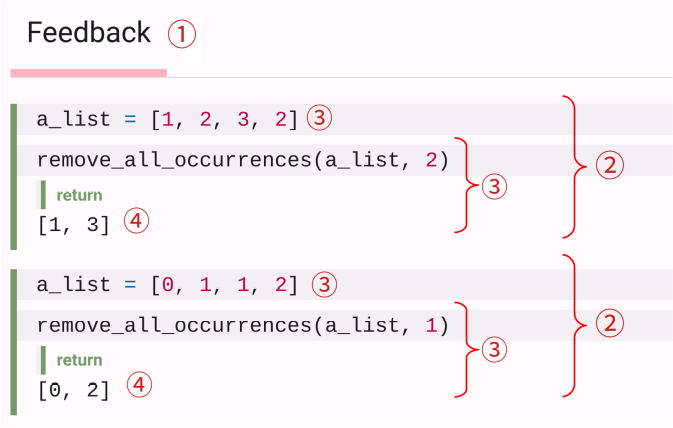
\includegraphics[scale=0.4]{dodona-rendering}
    \caption{A way to visually render the feedback (as done in Dodona resulting from evaluating a submission (in Python) with the test suite from TODO. There are four levels: \CircledText{1} units, \CircledText{2} testcases, \CircledText{3} tests and \CircledText{4} the scripts. Here, each testcase consists of two tests, the first of which has no script, while the second has one script (the expected return value).}
    \label{fig:dodona}
\end{figure}

TODO: add dataserialisation somewhere, perhaps own chapter

\section{Evaluating submissions}\label{sec:evaluating-submissions}

We now focus on the process TESTed performs when evaluating a submission~\cref{fig:flow}.
TODO fix figuur

The input for the evaluation process is a test suite and a submission, which is typically provided by the judge platform in which TESTed runs (or can be provided manually if TESTed is run on the command line).
TESTed then generates test code in the programming language of the submission, based on the test suite.
This is the bulk of language-specific code in TESTed, whose design and implementation are discussed in Programming-language-specific modules.

\subsection{Solvability and correctness checks}\label{subsec:solvability-and-correctness-checks}

The first step in the evaulation process is checking if the test suite is useable for the programming language of the submission.
This might not be the case for a number of reasons, the three main ones being:

\begin{itemize}
    \item The exercise designer has limited in which programming languages the exercise may be solved.
    \item The test suite uses constructs that are not supported by the programming language of the solution.
          For example, if the test suite uses object-oriented programming, the exercise will not be solvable in C or Haskell.
    \item The test suite contains programming-language-specific code but does not provide code for the programming language of the submission.
          For example, it is possible to manually provide the test code.
\end{itemize}

Additionally, there are some correctness checks, e.g.\ on the syntax of the test suite.

\subsection{Execution planning}\label{subsec:execution-planning}

The next step is planning the execution of the evaluation.
As discussed before, a test suite contains a number of testcases, which must be independent of each other.
This allows TESTed to implement optimisations to improve performance.

TESTed partitions the test suite into compilation units (a set of testcases that are compiled together), which are in turn partitioned into execution units (a set of testcases that are executed together).
While different compilation units cannot be executed as one execution unit, it is possible that one compilation unit represents multiple execution units.

\begin{figure}[h]
    \begin{subfigure}{\textwidth}
        \centering
        \includestandalone{planning-1}
        \caption{
            A schematic representation of the test suite.
            The test units are represented with green boxes, while the testcases (denoted as C\textsubscript{$n$}) are black boxes.
            In the subsequent figures, we leave the test suite box out to simplify the image.
        }
        \label{fig:planning-suite}
    \end{subfigure}
    \par\bigskip
    \begin{subfigure}{\textwidth}
        \centering
        \includestandalone{planning-2}
        \caption{
            The two possibilities for compilation units (denoted by red boxes).
            The upper scheme (with one compilation for the whole test suite) is always tried first.
            If this fails, each test unit becomes a compilation unit (the red boxes thus overlap with the green ones in the figure).
        }
        \label{fig:planning-compilation}
    \end{subfigure}
    \par\bigskip
    \begin{subfigure}{\textwidth}
        \centering
        \includestandalone{planning-3}
        \caption{
            Two possibilites execution unit partitionings (denoted by blue boxes), depending on the compilation units.
            In the first paritioning, there is a single compilation unit that is split into three execution units.
            The second partitioning cannot use the same execution units, as an execution unit cannot comprise multiple compilation units.
        }
        \label{fig:planning-execution}
    \end{subfigure}
    \caption{Schematic representation of the planning steps.}
\end{figure}

\subsubsection{Performance impact of the planning}

If performance was not relevant, the easiest execution plan would be to compile and execute each testcase individually.
After all, they are independent of each other, and separate compilation and execution would ensure that independence.

However, since this would be prohibitively slow (e.g.\ a test suite with fifty test cases would need fifty compilation steps and fifty execution steps),
TESTed has two goals when creating an execution plan, designed to improve the performance:

\marginnote{The final execution units are also executed in parallel, which is described in TODO.}
\begin{enumerate}
    \item Reducing the number of compilation units.
    \item Reducing the number of execution units.
\end{enumerate}

\subsubsection{Compilation units}

First, TESTed tries to use a single compilation unit for the whole test suite.
This is achieved by creating a program that accepts an argument to indicate the execution that should be run.

% TODO: introductie verbeteren hier
In programming languages without an explicit compilation step, the compilation is no more than a syntax check.
\marginnote{
    For example, our JavaScript implementation uses \texttt{node -c}.
}
In compiled languages, the compilation is often much stricter, for example, failing if a non-existing function is used.
This poses a problem for evaluating submissions: students might implement the first part of an exercise, without implementing a second part.
This would mean TESTed will not evaluate the already implemented functions, as the compilation step failed.

Therefore, if the compilation of the whole test suite fails, TESTed falls back to using one compilation unit per unit in the test suite.
Since a unit is a set of logically related testcases, this seems like a good compromise between fain-graind compilation (thus allowing more of the submission to be evaluated) and performance (the more compilation units, the slower the evaluation will be).

\subsubsection{Execution units}

Next, the compilation units from the previous steps are partitioned into execution units.
Each execution unit must be at least one compilation unit: we cannot execute multiple compilation units together.
However, depending on the testcases inside a compilation unit, we can (and do) execute a compilation unit multiple times.

For performance reasons, the ideal partitioning would be a single execution unit for the whole test suite.
However, this prevents certain types of exercises from being evaluated correctly.
Therefore, a new execution unit is started based on the type of testcase: if a testcase has stdin, command line arguments or an explicit check for the exit code, a new execution unit is started.

\subsection{Evaluation process}\label{subsec:evaluation-process}

We can now take a look at the complete evaluation process used by TESTed when evaluating a submission (a schematic is~\cref{fig:flow}).
First, the test suite is partitioned into compilation units, as described in~\cref{subsec:execution-planning}.
For each of these units, the relevant code is generated and the resulting test code is compiled.
If this compilation failed, TESTed returns to the planning step to try again with a different partitioning.
TODO: show this on the figure.

After compilation, each resulting executable contains one or more execution units.
These are then all executed, and the side effects (such as exceptions, stdout, stderr, etc.) and results (i.e.\ return values) are recorded.
These results are then checked for correctness against the test suite (see TODO).
This will result in the feedback that is finally given to submitter.

TESTed also has a step where static analyses is possible on the submission.
\marginnote{Examples include \texttt{ESLint}, \texttt{pylint} or \texttt{hlint}.}
Currently, all supported programming languages use this step to run a linter on the submission, the results of which are also included in the feedback as code annotations.







\begin{figure}
    \centering
    \includestandalone{flow}
    \caption{
        The evaluation process of TESTed.
        The input consists of a submission and a test suite.
        After the planning phase, test code is generated, compiled, and executed.
        These results are then checked, which produces the final feedback.
        Separately, a linter runs on the submission, and its results are also included in the feedback.
    }
    \label{fig:flow}
\end{figure}



\end{document}
